	\section{Цель работы}
		Изучить базовые понятия онтологического подхода и инструментальные средства онтологического проектирования, а также получить навыки работы с редактором онтологий Protégé.
		
	\section{Предметная область}
		Social Trading - онлайн-трейдинг на финансовых рынках в рамках социальной платформы, внутри которой трейдеры взаимодействуют друг с другом.
		
		Трейдеры получают возможность создавать и вступать в интернет-сообщества, чтобы создать социальную среду, где они могут получать информацию и следовать за другими «успешными» трейдерами одним нажатием кнопки. Участники делятся на 2 типа: ведущие трейдеры и ведомые трейдеры. Ведущие трейдеры делятся с ведомыми информацией и своими действиями на рынке, а ведомые могут как делать свои собственные действия с учётом полученной информации, так и просто повторять за авторитетным трейдером. 
		
		Цель разрабатываемой онтологии: по известным транзакциям пользователей выявить наличие отношений следования между ними.
		
	\newpage
	\section{Порядок выполенения работы}
		\subsection{Структура онтологии}
			Для решения задачи необходимо спроектировать базу понятий, атрибутов и связей, отражающих структуру предметной области. 
			
			Выделим 2 основных класса:
			\begin{enumerate}
				\item Пользователь - трейдер. Трейдер может следовать за другим трейдером и копировать его транзакции. 
				\item Транзакция - акт финансового взаимодействия пользователя с рынком. В рамках данной работы каждая транзакция имеет свою <<ставку>> на повышение или понижение стоимости того или иного актива, а также время создания в часах.
				Транзакция может быть скопирована с другой транзакции.
			\end{enumerate}
		
			Описанные понятия и их связи изображены на рис. \ref{fig:ontograph}.
			
			\begin{figure}[h]
				\centering
				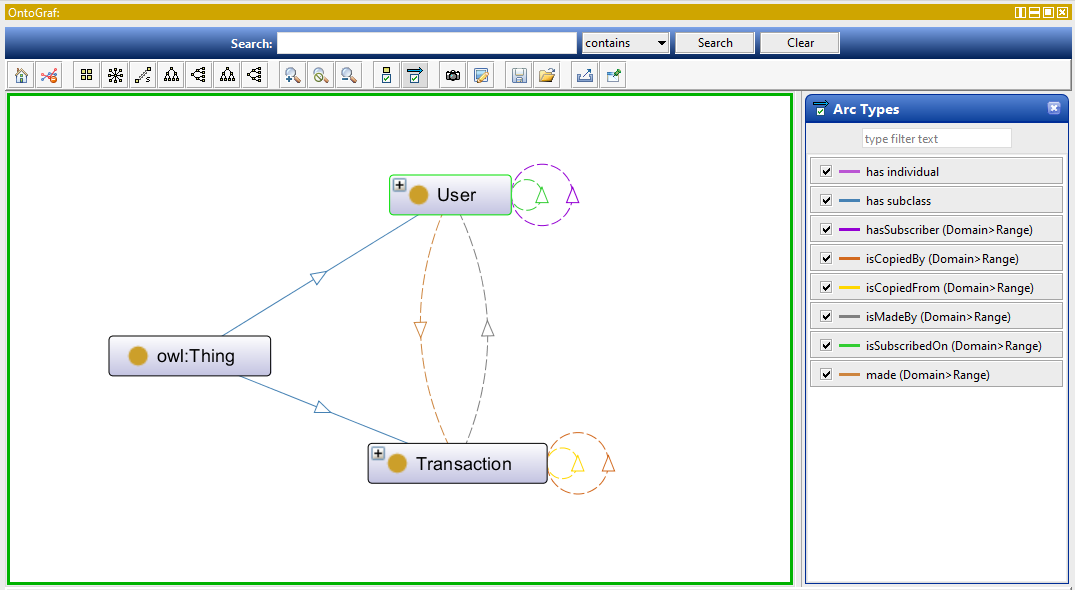
\includegraphics[width=\linewidth]{ontograph}
				\caption{Структура онтологии, визуализированная с помощью OntoGraph.}
				\label{fig:ontograph}
			\end{figure}
		
		\newpage
		\subsection{Правила вывода}
			Для начала необходимо вывести факт копирования транзакцией другой транзакции. Транзакция считается скопированной с другой транзакции, если она сделана в течение двух часов после первой и обе транзакции имеют одинаковую <<ставку>>. Данное правило реализовано средствами встроенного редактора SWRL правил.
			
			\begin{lstlisting}
Transaction(?x) ^ Transaction(?y) ^ differentFrom(?x, ?y) ^ bet(?x, ?x_bet) ^ bet(?y, ?y_bet) ^ swrlb:equal(?x_bet, ?y_bet) ^ hour(?x, ?x_hour) ^ hour(?y, ?y_hour) ^ swrlb:greaterThan(?x_hour, ?y_hour) ^ swrlb:subtract(?diff, ?x_hour, ?y_hour) ^ swrlb:lessThanOrEqual(?diff, 2) -> isCopiedFrom(?x, ?y)
			\end{lstlisting}
			
			Пользователь следует за другим пользователем, если у первого есть транзакции, скопированные с транзакций второго.
			
			\begin{lstlisting}
isCopiedFrom(?x, ?y) ^ isMadeBy(?x, ?x_user) ^ isMadeBy(?y, ?y_user) ^ differentFrom(?y_user, ?x_user) -> isSubscribedOn(?x_user, ?y_user)
			\end{lstlisting}
			
			Вдобавок, связь следования между пользователями по своей сути транзитивна, т.к. явно следуя за одним человеком, участник видит и действия, скопированные им у других трейдеров. Опишем эту транзитивность следующим правилом.
			\begin{lstlisting}
Transaction(?x) ^ isCopiedFrom(?x, ?y) ^ isCopiedFrom(?y, ?z) -> isCopiedFrom(?x, ?z)
			\end{lstlisting}
			
	\section{Пример работы}
		Для проверки правил вывода создадим 3-х пользователей и 4 транзакции. Их явные связи изображены на рис. \ref{fig:instances-before}.
		
		\begin{figure}[h]
			\centering
			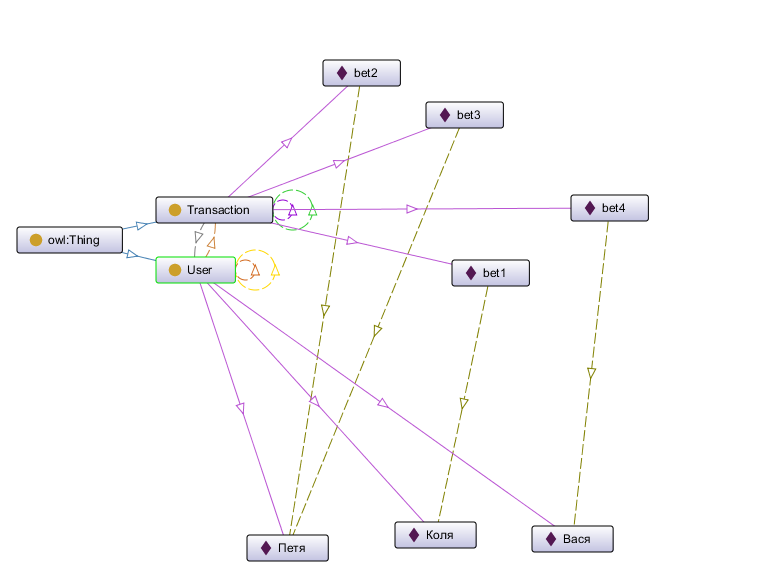
\includegraphics[width=\linewidth]{instances-before}
			\caption{Исходные данные для проверки правил вывода.}
			\label{fig:instances-before}
		\end{figure}
		\FloatBarrier
		
		На рис. \ref{fig:output} приведены начальные данные объектов (выделены жирным шрифтом) и данные, выведенные с помощью SWRL правил Reasoner'ом <<Pellet>>. 	
	
		\begin{figure}[ht]
			\begin{minipage}[ht]{0.49\linewidth}
				\center{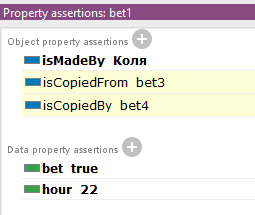
\includegraphics[width=0.8\linewidth]{bet1} \\ а) bet1}
			\end{minipage}
			\hfill
			\begin{minipage}[ht]{0.49\linewidth}
				\center{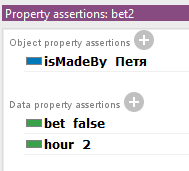
\includegraphics[width=0.8\linewidth]{bet2} \\ б) bet2}
			\end{minipage}
			\vfill
			\begin{minipage}[ht]{0.49\linewidth}
				\center{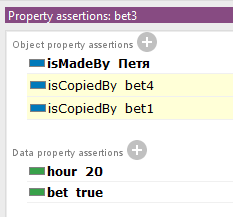
\includegraphics[width=0.8\linewidth]{bet3} \\ в) bet3}
			\end{minipage}
			\hfill
			\begin{minipage}[ht]{0.49\linewidth}
				\center{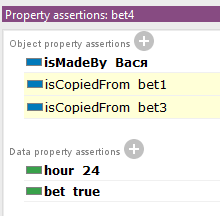
\includegraphics[width=0.8\linewidth]{bet4} \\ г) bet4}
			\end{minipage}
			\vfill
			\begin{minipage}[ht]{0.49\linewidth}
				\center{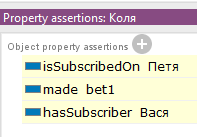
\includegraphics[width=0.8\linewidth]{kolya} \\ д) Коля}
			\end{minipage}
			\hfill
			\begin{minipage}[ht]{0.49\linewidth}
				\center{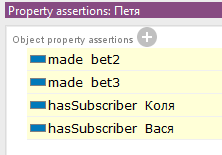
\includegraphics[width=0.8\linewidth]{petya} \\ е) Петя}
			\end{minipage}
			\vfill
			\center{
				\begin{minipage}[ht]{0.49\linewidth}
					\center{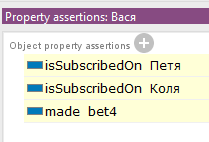
\includegraphics[width=0.8\linewidth]{vasya} \\ ж) Ваня}
				\end{minipage}
			}
			\vfill
			\caption{Параметры тестовых объектов.}
			\label{fig:output}  
		\end{figure}
		\FloatBarrier
	
	
		
	\section{Вывод}
		В процессе выполнения работы изучены базовые понятия онтологического подхода и инструментальные средства онтологического проектирования, а также получить навыки работы с редактором онтологий Protégé. Создана онтология <<Social Trading>>. Для неё созданы и протестированы правила вывода знаний на языке SWRL.